\title{Ground survey to assess hemlock sawfly population during a large-scale outbreak in Southeast Alaska}

\subtitle{\doi{10.----------}}

\author{by Elizabeth Graham\footnote{USDA Forest Service R10, Forest Health Protection}}

\maketitle

\begin{figure}[H]
\begin{center}
%\vspace{2mm}
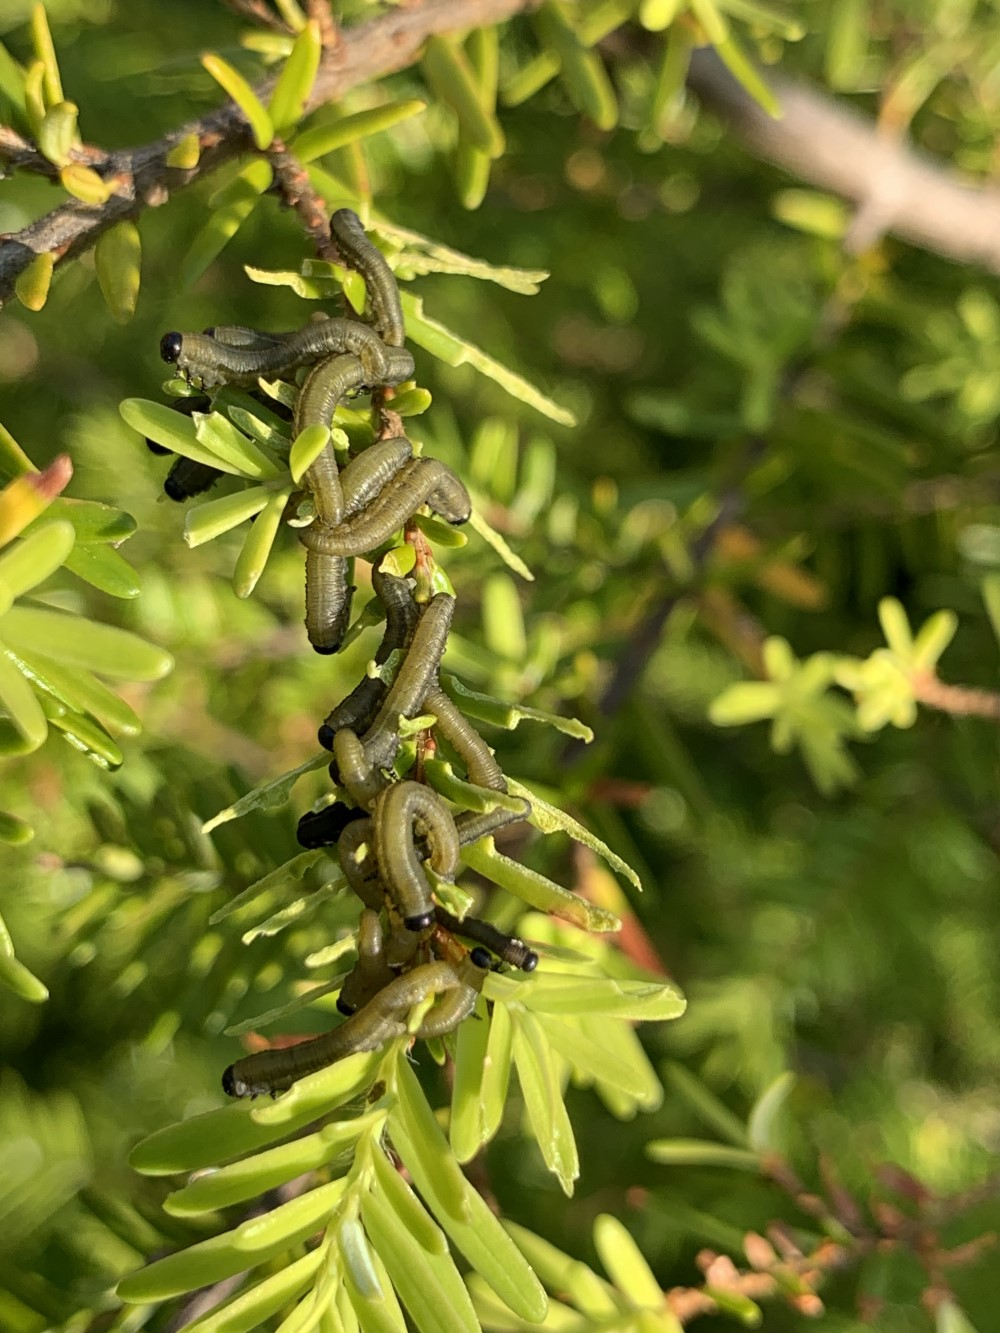
\includegraphics[width=\textwidth]{img/hemlock_sawfly_larvae.jpg}
\caption{Aggregate of hemlock sawfly feeding on western hemlock.}
\label{hemlock_sawfly_larvae}
\end{center}
\end{figure}

\section{Introduction}

Hemlock sawfly (Hymenoptera: Diprionidae \textit{Neodiprion tsugae}, Figure \ref{hemlock_sawfly_larvae}) is an important defoliator of hemlock (\textit{Tsuga} spp.)  throughout its range from the panhandle of Southeast Alaska through coastal British Columbia, Washington and Oregon as well as in Interior British Columbia, Idaho and Montana \citep{Hardetal1976}.  Significant outbreaks have been recorded during aerial detection surveys in Southeast Alaska since the mid-1960’s (Figure \ref{hemlock_sawfly_damage_graph}) and there were reports of a major outbreak impacting all of the Tongass National Forest during the mid-1950’s. Western hemlock (\textit{Tsuga heterophylla}) is the preferred host, however they also feed on mountain hemlock (\textit{Tsuga mertensiana}) as well as Sitka spruce (\textit{Picea sitchensis}) and occasionally other conifers.  The larvae feed on the older needles, avoiding the new growth, often only eating half of the needle, a feeding pattern called “wasterful feeding” (Figure \ref{hemlock_sawfly_wasteful_feeder}).  Because the important new foliage is retained feeding damage from hemlock sawfly rarely result in mortality, though it can result in topkill and reduction in radial growth.  Mortality can occur when outbreaks of hemlock sawfly coincide with a western blackheaded budworm outbreak (\textit{Acleris gloverana}, Figure \ref{western_blackheaded_budworm_larva}), which feed in the buds and new foliage resulting in complete defoliation. 

\begin{figure}[H]
\begin{center}
\vspace{4mm}
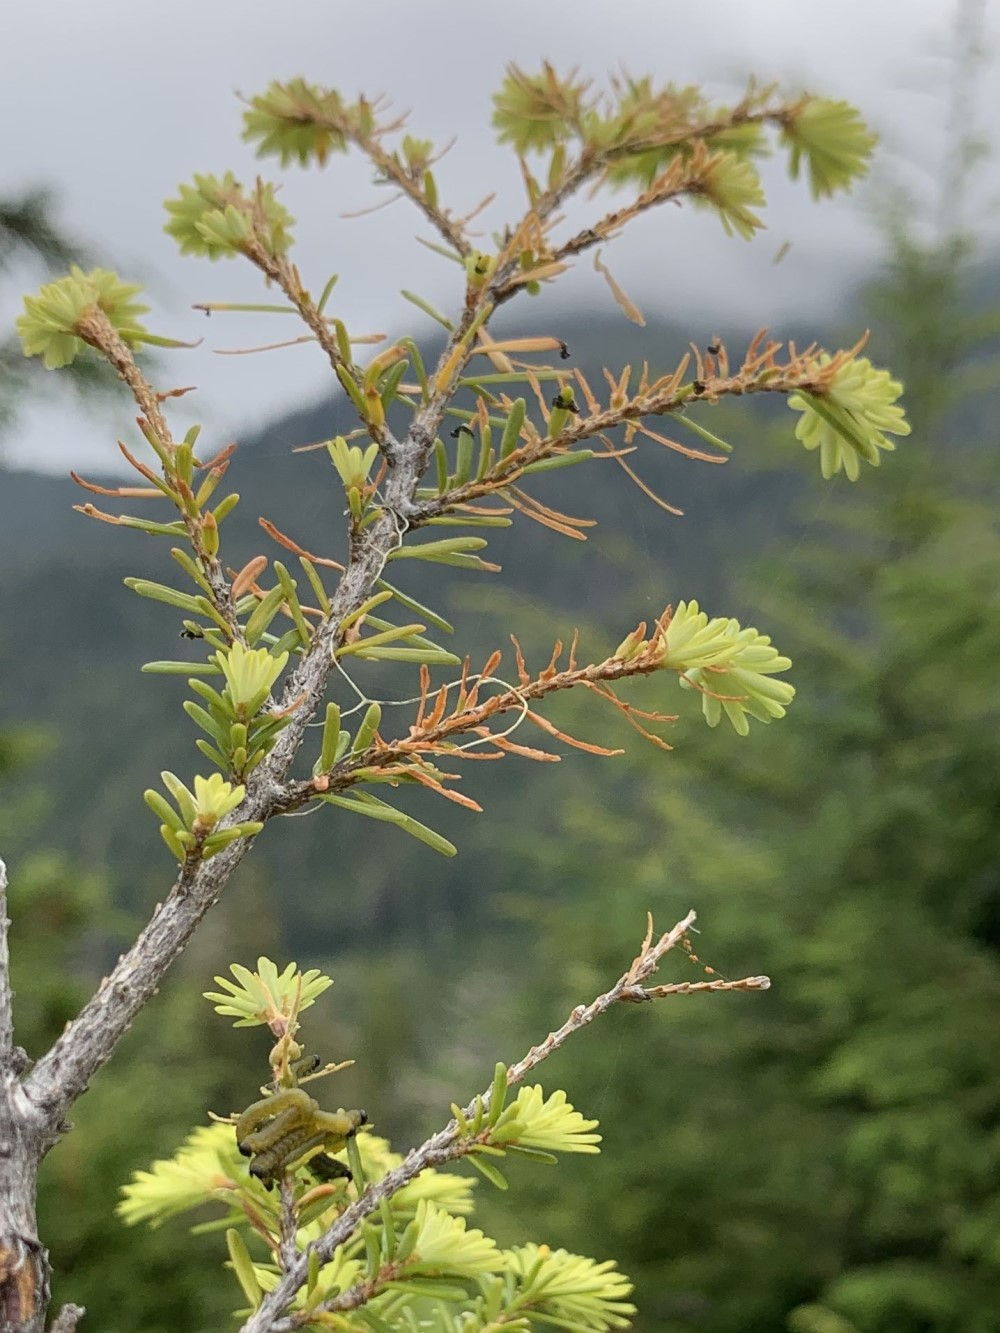
\includegraphics[width=\textwidth]{img/hemlock_sawfly_wasteful_feeder.jpg}
\caption{Hemlock sawfly larvae preferentially feed on older needles, usually leaving the new growth untouched.}
\label{hemlock_sawfly_wasteful_feeder}
\end{center}
\end{figure} 

\end{multicols}
\begin{figure}[H]
\begin{center}
%\vspace{2mm}
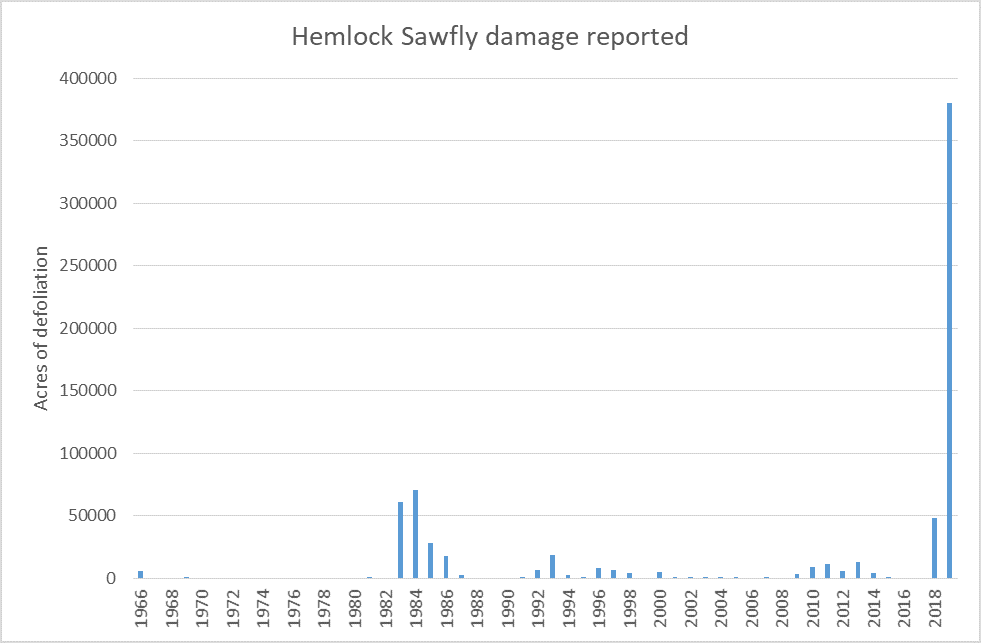
\includegraphics[width=16cm]{img/hemlock_sawfly_damage_graph.png}
\caption{Hemlock sawfly defoliation recorded during annual aerial detection survey since 1966.}
\label{hemlock_sawfly_damage_graph}
\end{center}
\end{figure} 
\begin{multicols}{2} 

\begin{figure}[H]
\begin{center}
\vspace{2mm}
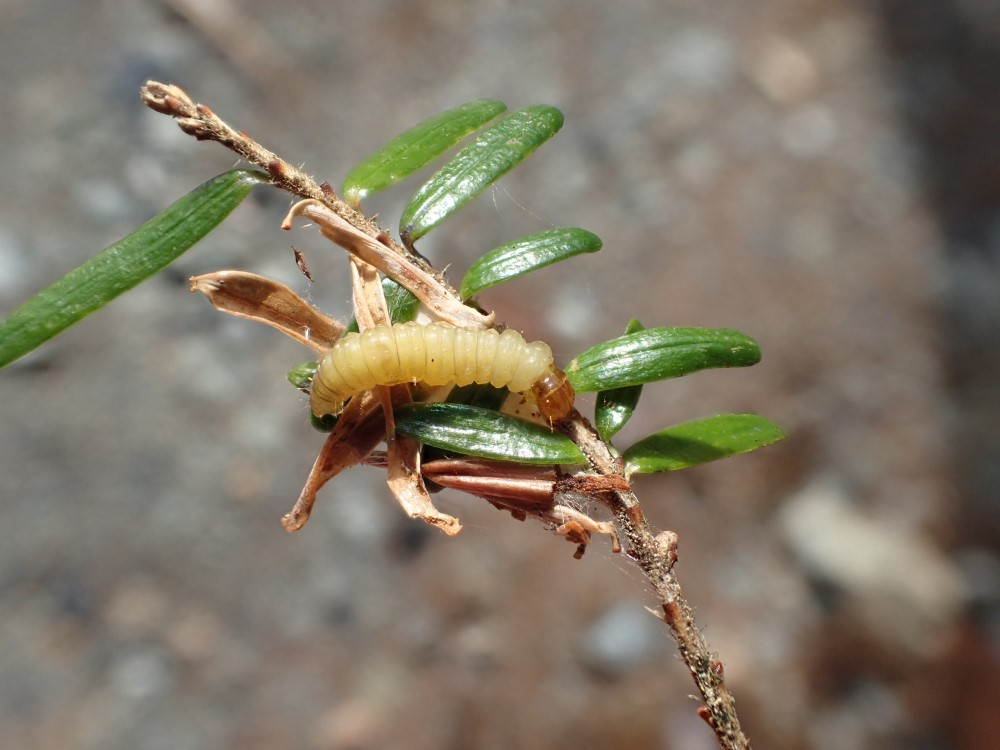
\includegraphics[width=\textwidth]{img/western_blackheaded_budworm_larva.jpg}
\caption{Western blackheaded budworm found on a western hemlock in Juneau, Alaska.}
\label{western_blackheaded_budworm_larva}
\end{center}
\end{figure} 

The current hemlock sawfly outbreak started in Southeast Alaska in 2018.  During our annual aerial detection surveys, defoliation was observed on >48,000 acres of western hemlock.  In 2019 the damage rose to >380,000 acres (Figure \ref{hemlock_sawfly_defoliation}) and was often concentrated on southern to western facing aspects (Figure \ref{hemlock_sawfly_defoliation_2}). Outbreaks are closely connected to climate conditions and can be triggered during drier than normal conditions due to a reduction in entomopathogenic fungi, one of the factors that help maintain population levels.   Southeast Alaska exhibited warmer and drier than average summer conditions in both 2018 and 2019 which limited entomopathogenic fungal growth, allowing larval populations to build to outbreak. In response to the outbreak, a systematic ground survey to sample defoliator populations on hemlock was conducted throughout Southeast Alaska in 2019.  The objectives of the survey were to record the species and number of defoliators found on hemlock trees as well as the amount of feeding damage and any other factors that may have an impact hemlock sawfly populations.

\section{Methods}

Ground surveys were conducted between June 26\textsuperscript{th} and July 23\textsuperscript{rd} 2019, starting in Ketchikan, followed by Prince of Wales, Mikof, Kupreanof, Zarembo, and Wrangell Islands ending with Sitka and Juneau.  Due to time and budget constraints, surveys were limited to areas with accessible road systems.  Plot points were randomly created in Arc\acr{GIS} using the Forest Service road system and a hemlock component as requirements.  Actual plot locations were placed within a \nicefrac{1}{4} mile buffer of the randomly generated points, where host tree accessibility was the greatest.  Areas with no hemlock or were inaccessible were eliminated and the next randomized location was used.   At each location the plot center was recorded as well as the azimuth from the road.  Plot level data consisted of forest canopy class and forest type. For individual trees, \acr{DBH} and crown ratings were recorded. Defoliators were sampled using a 28” square canvas beating sheet, onto which the surveyor knocks insects from branches (Figure \ref{beating_sheet}).  The number of hemlock sawfly and western blackheaded budworm were recorded by range (<10, 10-20, >20); any other additional defoliators were also recorded.  Hemlock sawflies with fungal infections were recorded separately from healthy sawflies.  Hemlock sawfly pupae were also recorded.  There were no infected western blackhead budworm or pupae observed. 

\section{Results}
 
In total, 76 ground plots were surveyed for hemlock defoliators throughout Southeast Alaska, of those 70 plots had hemlock sawfly larvae present (Figure \ref{hemlock_sawfly_plot_map}).  Defoliation was the greatest on Mitkof and Kupreanof Islands, in areas where the outbreak was in its second year (Figure sawfly ground surveys).  Those two islands also had the highest proportion of trees with sawflies and a high abundance rating.  Prince of Wales Island, which is in its first year of an outbreak had a lower amount of defoliation but a high abundance of sawflies in the plots. Hemlock sawfly activity was lowest on Revillagigedo and Baranof Islands.   The results of our ground surveys align closely with the amount of damage mapped during our aerial detection survey in those areas (see Dubois article). 

\begin{figure}[H]
\begin{center}
\vspace{2mm}
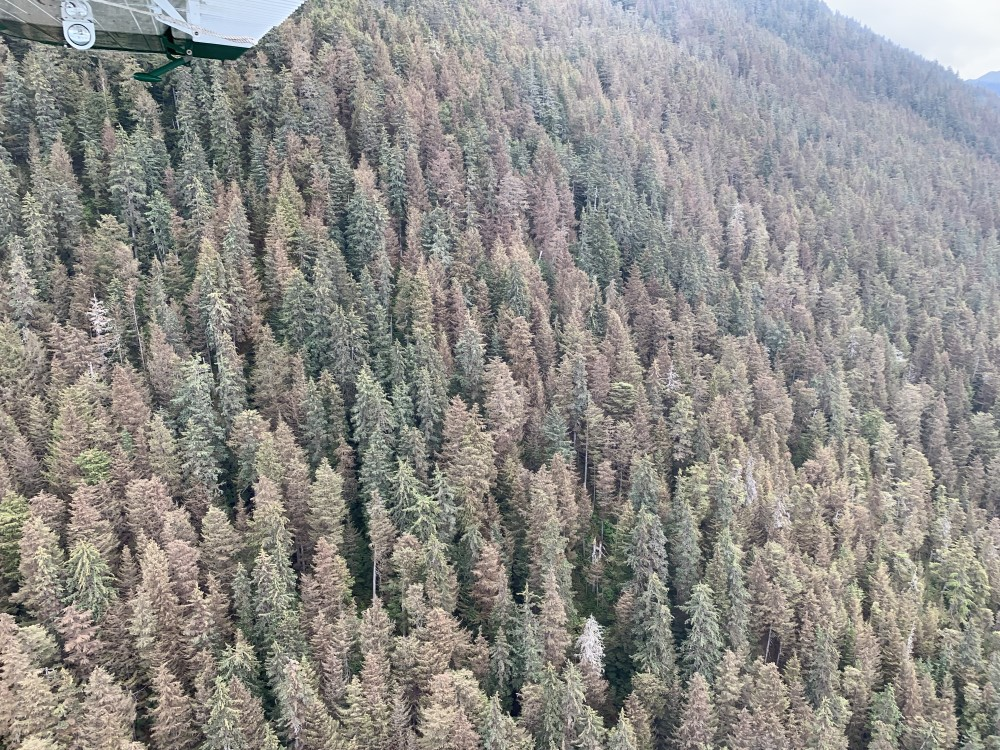
\includegraphics[width=\textwidth]{img/hemlock_sawfly_defoliation.jpg}
\caption{Heavily defoliated western hemlock as seen during aerial detection survey.}
\label{hemlock_sawfly_defoliation}
\end{center}
\end{figure} 

\begin{figure}[H]
\begin{center}
\vspace{2mm}
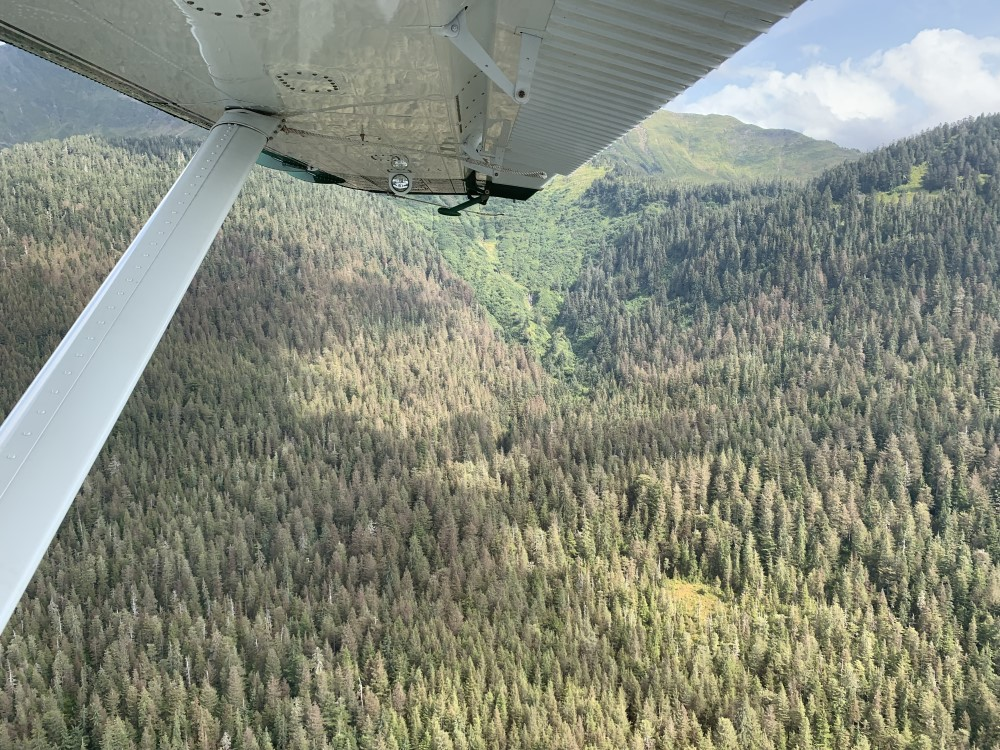
\includegraphics[width=\textwidth]{img/hemlock_sawfly_defoliation_2.jpg}
\caption{Defoliation was heaviest on southern and western facing aspects as well as along river drainages.}
\label{hemlock_sawfly_defoliation_2}
\end{center}
\end{figure} 



  
\begin{figure}[H]
\begin{center}
\vspace{2mm}
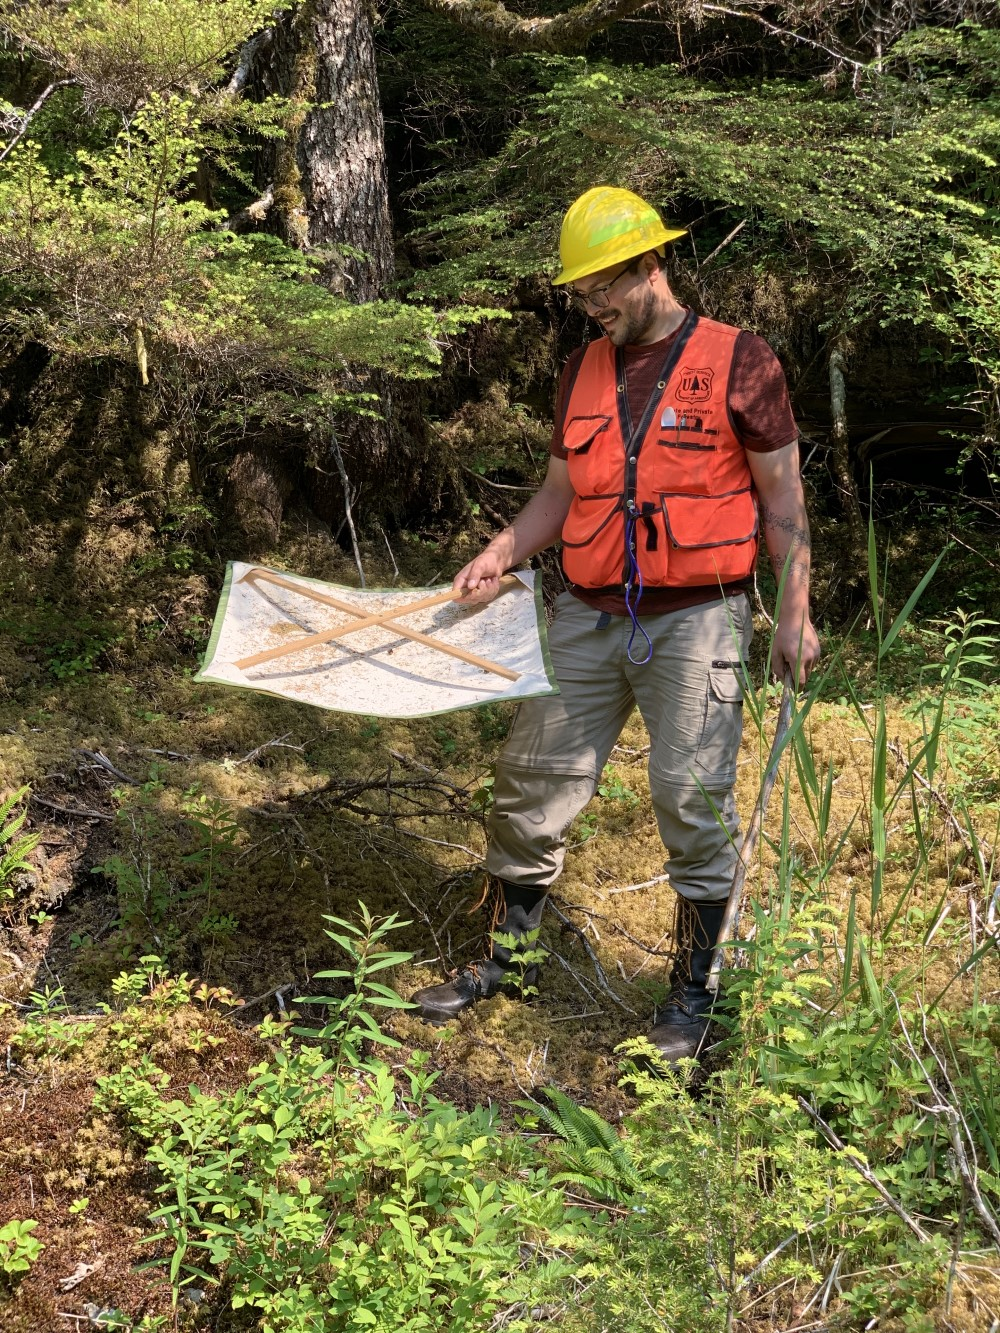
\includegraphics[width=\textwidth]{img/beating_sheet.jpg}
\caption{Forest Service Biotech Isaac Davis uses a beating sheet to sample for defoliating insects on hemlock trees.}
\label{beating_sheet}
\end{center}
\end{figure} 


\end{multicols}
\begin{figure}[H]
\begin{center}
%\vspace{2mm}
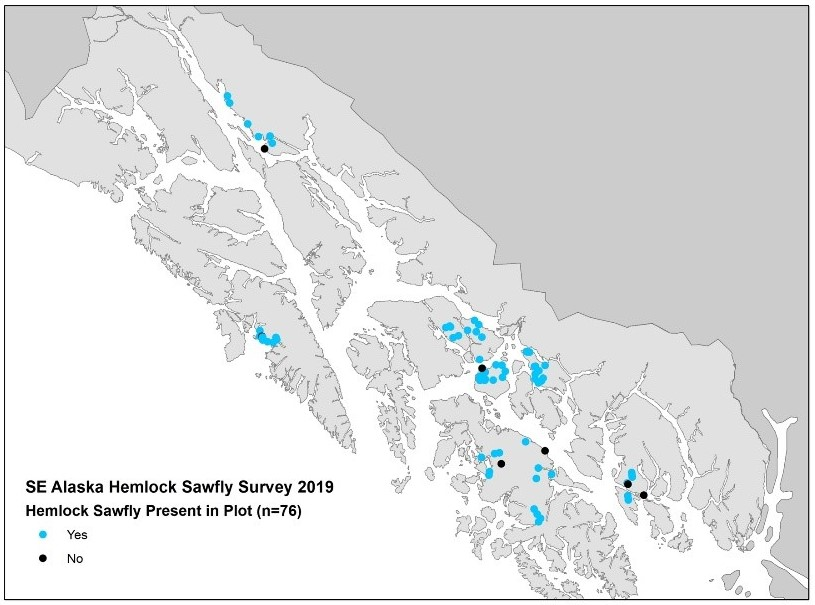
\includegraphics[width=16cm]{img/hemlock_sawfly_plot_map.jpg}
\caption{Locations of hemlock defoliator ground plots, plots marked as blue had hemlock sawfly whereas black did not.}
\label{hemlock_sawfly_plot_map}
\end{center}
\end{figure} 
\begin{multicols}{2} 

 
Other species of defoliating insects collected on the beating sheets were also recorded during the survey.  The most commonly encountered defoliators were western blackheaded budworm and Geometrid caterpillers.  Western blackheaded budworm was found in 38 of the 76 plots however the proportion of trees with budworm was consistently low as was their abundance rating.  No other species of defoliator were found as consistently or in high enough abundance to cause any notable damage. 
 
The highest amount of hemlock sawfly larvae infected with entomopathogenic fungi was found on Mitkof and Kupreanof Islands, areas in their second year of hemlock sawfly outbreak.  Pupal cases collected during the fall from Mitkof Island also had a high parasitism rate.


\bibliography{hemlock_sawfly}

